% fig_island_ndz.tex
% TR-39: Non-detection zone in (ΔP, ΔQ) load-mismatch space
%
% Passive NDZ: |ΔP| < 0.020 pu  AND  |ΔQ| < 0.050 pu
% Active (Q-injection) reduces ΔQ NDZ significantly
% Combined NDZ shown as reduced rectangle

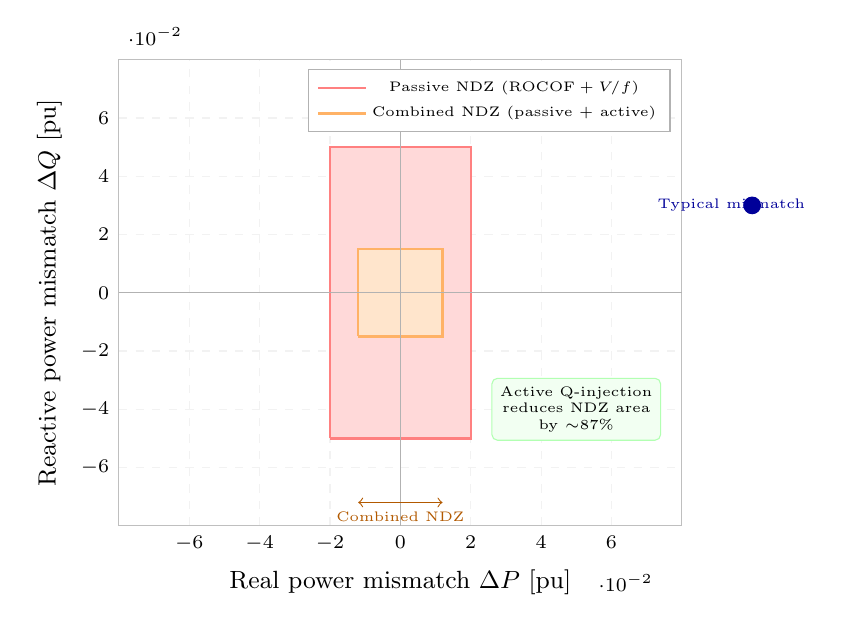
\begin{tikzpicture}
\begin{axis}[
  name         = ndzax,
  width        = 0.72\textwidth,
  height       = 7.5cm,
  xlabel       = {Real power mismatch $\Delta P$ [pu]},
  ylabel       = {Reactive power mismatch $\Delta Q$ [pu]},
  xlabel style = {font=\small},
  ylabel style = {font=\small},
  xmin=-0.08, xmax=0.08,
  ymin=-0.08, ymax=0.08,
  xtick        = {-0.06,-0.04,-0.02,0,0.02,0.04,0.06},
  ytick        = {-0.06,-0.04,-0.02,0,0.02,0.04,0.06},
  xticklabel style={font=\scriptsize},
  yticklabel style={font=\scriptsize},
  tick style   = {draw=none},
  axis line style={gray!50},
  grid         = major,
  grid style   = {gray!10, dashed},
  legend style = {at={(0.98,0.98)}, anchor=north east, font=\tiny,
                  draw=gray!60, fill=white},
  clip=false,
]

%% Passive NDZ rectangle: |ΔP|<0.020, |ΔQ|<0.050
\addplot[red!20, fill=red!15, draw=red!50, thick]
  coordinates {(-0.020,-0.050) (0.020,-0.050)
               (0.020, 0.050) (-0.020, 0.050) (-0.020,-0.050)};
\addlegendentry{Passive NDZ ($\mathrm{ROCOF}+V\!/f$)}

%% Combined NDZ (active + passive): |ΔP|<0.012, |ΔQ|<0.015
\addplot[orange!30, fill=orange!20, draw=orange!60, thick]
  coordinates {(-0.012,-0.015) (0.012,-0.015)
               (0.012, 0.015) (-0.012, 0.015) (-0.012,-0.015)};
\addlegendentry{Combined NDZ (passive + active)}

%% Detection region markers — typical operating point
\addplot[blue!60!black, only marks, mark=*, mark size=3pt]
  coordinates {(0.10, 0.03)};
\node[blue!60!black, font=\tiny, right=3pt] at (axis cs:0.068, 0.03)
  {Typical mismatch};

%% Axes through origin
\draw[gray!60, thin] (axis cs:-0.08,0) -- (axis cs:0.08,0);
\draw[gray!60, thin] (axis cs:0,-0.08) -- (axis cs:0,0.08);

%% Dimension annotations
\draw[<->, orange!70!black, thin]
  (axis cs:-0.012, -0.072) -- (axis cs:0.012, -0.072)
  node[midway, below, font=\tiny] {Combined NDZ};

\draw[<->, red!60!black, thin]
  (axis cs:-0.020, 0.065) -- (axis cs:0.020, 0.065)
  node[midway, above, font=\tiny] {Passive NDZ};

%% Reduction annotation
\node[draw=green!30, fill=green!5, rounded corners=2pt,
      font=\tiny, inner sep=3pt, align=center]
  at (axis cs:0.05, -0.04)
  {Active Q-injection\\reduces NDZ area\\by $\sim$87\%};

\end{axis}
\end{tikzpicture}
